\section{II. Thinning/Skelettierung}
\subsection{Grundlagen}
\begin{frame}{Thinning}
\begin{center}
 Idee: Man nehme den kompletten freien Raum (Flure, Räume), und wende darauf einen thinning-Algorithmus an.
 \bigbreak
 
 Dann bleibt ein Skelett, dem Voronoi sehr ähnlich, übrig.
 
 \end{center}
\end{frame}

\begin{frame}{Thinning}

\begin{figure}[h]
 \centering
 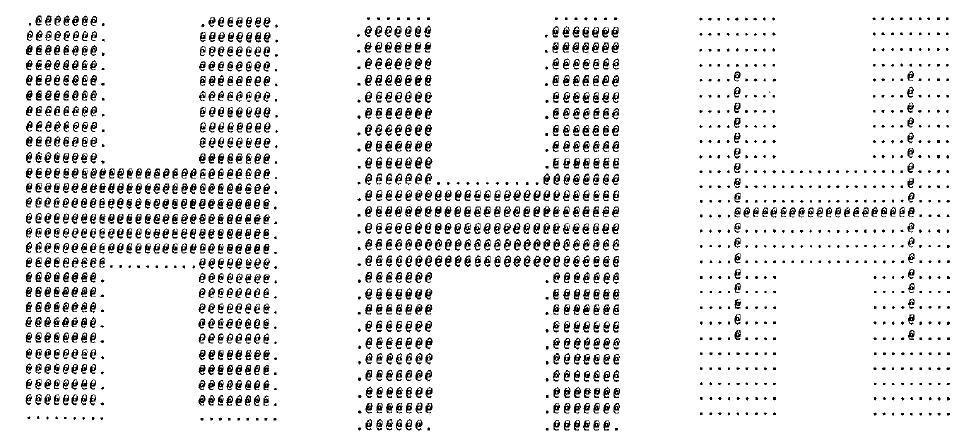
\includegraphics[width=0.65\textwidth]{./material/thinning1.png}
 % complete.png: 845x703 pixel, 72dpi, 29.81x24.80 cm, bb=0 0 845 703
 \caption{Thinning \cite{ZhangSuen}}
 \label{fig:gesamt}
\end{figure}
 
\end{frame}

\begin{frame}{Thinning-Bedingungen}

\begin{columns}\begin{column}[l]{0.4\textwidth}

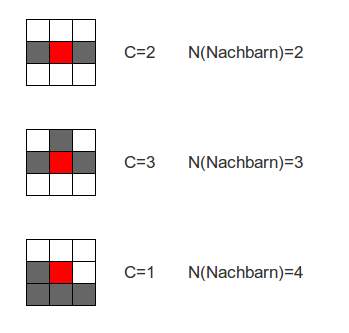
\includegraphics[width=1.0\textwidth]{./material/thinning2.png}

\end{column}
\begin{column}[r]{0.6\textwidth}
 \pause
 \begin{enumerate}
  \item Aktuelle Zelle ist belegt
  \item Connectivity $ = 1$
  \item $2 \leq $ Anzahl der Nachbarn $ \leq 6$
  \item Weitere Bedingungen nach Ausprägung des Algorithmus'
 \end{enumerate}
 
\end{column}
\end{columns}
 
\end{frame}
\begin{frame}
 Berechnung der kritischen Punkte und Linien analog zu Voronoi.

\end{frame}

\subsection{Screencast}
\begin{frame}
 \centering
 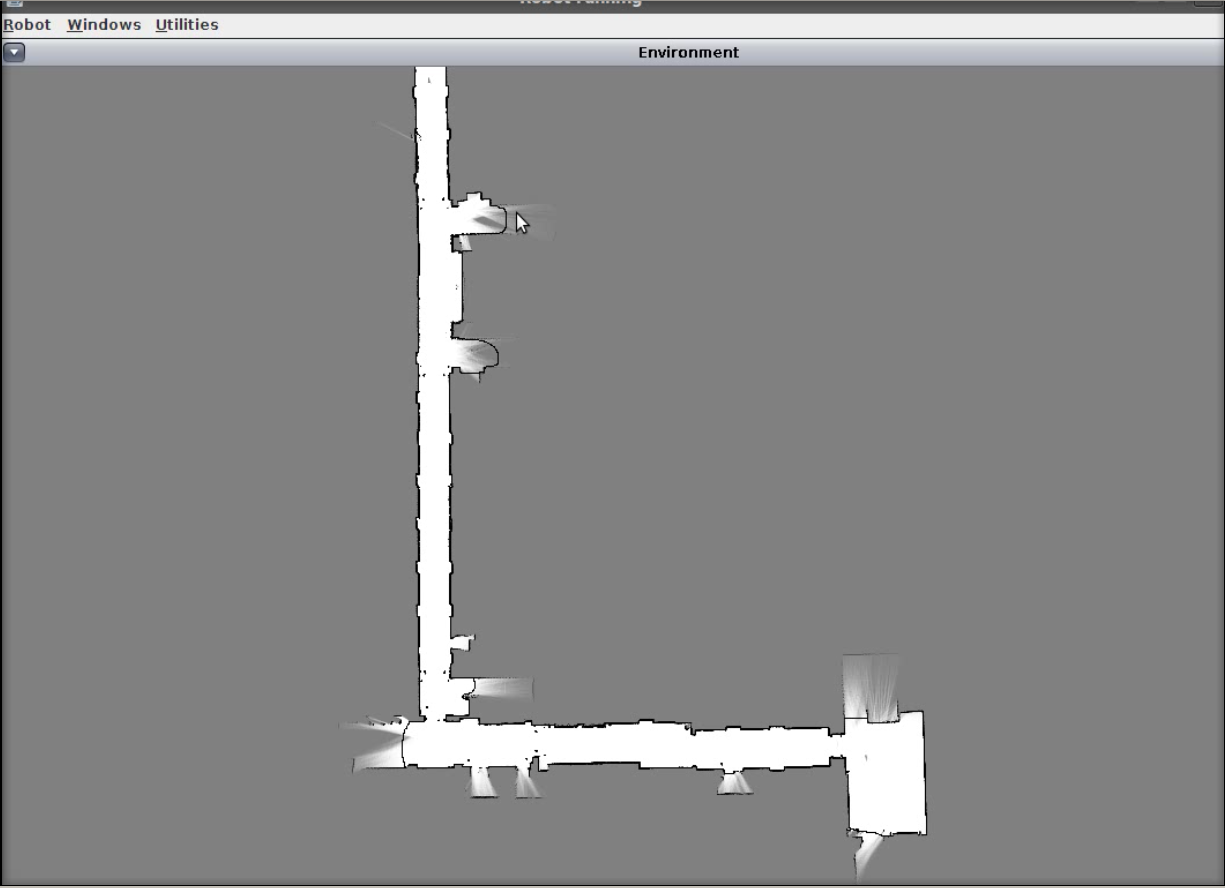
\includegraphics[width=0.85\textwidth]{./material/screencast.png}
\end{frame}

